%===================================== CHAP 3 =================================

\chapter{Implementation}\label{implementation-chap}

The chapter thoroughly described the implementation process and the implementation itself of both the visualization tool and the creation and training of the networks implemented for the case study.

\section{Visualization Tool}

In this section we will present the implementation details of the visualization tool created as a part of this thesis. We start with a summary of the related results from the Specialization Project, before explaining the system development methodology used in the implementation process. Then, we will present the two quality attributes that have been a focus through the design and implementation, and state our decisions regarding the technology used. Finally, we will showcase the implementation details for the main parts of the implemented visualization tool.

\subsection{Prototype}

This section presents the results from the Specialization Project in terms of the already implemented prototype of the visualization tool, as well as some pointers on the planned improvements and extensions to be done for this thesis.

\subsubsection{Description}

% Should say something about what kind of application it is, e.g. desktop vs web and why.
% --> desktop application, but runs in a web browser
% Also explain why there is a user system?

\noindent The prototype provides all the basic user functionality for creating a user, and logging in and out, including validation of user name and password. A user can upload Python scripts from their computer to the server, and tag them with various topics to make them easier to search for, using the search bar on the page showing all uploaded scripts. \\

\noindent By selecting a specific script, the user can view the code, add tags to, delete, and of course run, the script. A separate menu tab for visualizations provides the user with visualizations of the data produced while running. The only visualization techniques implemented are the training progress and layer activations laid out after each other on a single page. The training progress includes two separate plots showing accuracy and loss over batch, while the layer activations are shown for each single layer of the network defined in the script.

\subsubsection{Planned Improvements and Extensions}

The overall purpose will be to add more functionality with the goal of improving the user's understanding of the network. This may be new visualization techniques, training process statistics, better presentations of data, and more user controls. Another useful addition can be allowing the user more flexibility and make the visualizations more interactive.

\subsection{System Development Methodology}

The development of the visualization tool has been carried out by a team consisting of the two of us, with no specific set of roles. Because of the small team size, we did not see the need for a dedicated project manager. Both of us were involved in designing the architecture and interface, as well as implementing and testing the system, giving us great knowledge of the whole system. Still, we maintained an efficient workflow by dividing the programming task into two main responsibility areas, one for each of us:
\begin{enumerate}
    \item Visualizing data using the selected visualization library and incorporating these into the user interface
    \item Implementing visualization techniques and creating networks to illustrate the use of the tool with the chosen deep learning library
\end{enumerate} % maybe add a sentence explaining that these areas were just pointers, and that we both did work on both areas.

\noindent The development process itself did not follow any strict guidelines, but included several elements from Agile methods. It has been an iterative and incremental process, starting with the existing prototype of the system that only implemented two of the visualization techniques in a very simple manner. Based on our own testing as well as feedback from our supervisors, functionality were added and adjustments were made in order to obtain a new and improved prototype. This process was repeated until we reached a satisfactory system according to the initial requirements. An example of the iterative part of the process is when we decided to replace the old visualization library with a new one that better suited our needs. An example of the incremental part of the process is when our supervisors expressed the wish for a way for the user to be able to upload an image to be used in producing some of the visualizations. Other concepts from Agile development that were put into use are code review, pair programming, and the use of a backlog to get an overview of the requirements.

\subsection{Focus Quality Attributes}

In addition to functional requirements, we wanted to incorporate some non-functional requirements as well. Thus we have selected two quality attributes that we consider to be of highest importance. Quality attributes are overall factors that represents areas of concern impacting the application as a whole. In our case, we have determined that the most important factors are as follows.

\subsubsection{Modifiability}

An important aspect of the system design of the visualization tool is to make sure that any part can be easily replaced. For instance, it should not be too difficult to alter the system to use a different deep learning library than the one employed in our implementation. This requires thorough consideration when designing the architecture, and typically calls for a module-based architecture with each module being loosely coupled, meaning that it should interact with as few of the other modules as possible.

\subsubsection{Usability}

Not only should the interface be simple and easy to navigate for the user, but the actual installation of the program and the adaption of the user's deep learning scripts to the tool, should be without much trouble. A thorough user manual and documentation of the API is the key to obtaining this kind of usability. Preferably, we would want any ANN to run in our program without problems, but it is near to impossible to generalize this much. The main goal was thus to support the most commonly used networks, but at the same time, as the previous section mentions, easily allow for extending the system to work with different kinds of ANNs.

\subsection{Technology Decisions}

This section presents the technology used in our implementation, as well as a justification of why they were selected and an identification of any potential drawbacks.

\subsubsection{Flask}

Flask is a web framework written in Python, used to build simple web applications. It is a micro-framework, meaning that it has very few dependencies to external libraries. It provides you with only the basic tools needed to create a web application, and is therefore very lightweight. There exists many plugins that can be added for an increased range of functionality. Since the focus of our visualization tool is not the web page itself, but rather its capabilities in terms of visualization techniques, Flask is the perfect choice. It allowed us to quickly set up an application and implement a basic user system and upload functionality.

\subsubsection{SQLite}

SQLite is a simple and lightweight relational SQL database engine. In contrast to many other databases, it is embedded into the application. It is often used to provide local data storage for desktop applications. An embedded database improves application performance, reduces cost and complexity, and improves reliability. Since we do not require any advanced database functionality, nor do we need to store large amounts of data or have many database connections at the same time, SQLite is a perfect choice for out visualization tool. It is uncomplicated to set up, and can also be easily replaced with a more advanced database system at a later time if needed.

\subsubsection{Keras}

Keras is a high-level neural networks library that can run on top of either TensorFlow or Theano. Its purpose is to provide a way to quickly and easily create models and start experimenting. It is very minimalistic, providing only enough to achieve an outcome, while still allowing for extensibility by making it easy to add and use new modules within the framework. Keras provides the user with several callbacks, i.e. sets of functions to be applied at giving stages of the ANN training procedure. It also allows for creating your own custom callbacks, which is perfect for our use case, since we then can create callbacks that produces the data needed for each visualization technique. Consequently, we have chosen to adapt our visualization tool specifically to Keras. We have added support for both the TensorFlow and the Theano backend. However, we have concentrated on TensorFlow, thus not all visualizations have been extensively tested for the Theano backend.

\subsubsection{Bokeh}

Bokeh is a Python interactive visualization library for modern web browsers. It can easily be embedded into a Flask application, as we will demonstrate later in this chapter. The library is simple in use, and has the flexibility of adding interactions and highly advanced customization. Another benefit is that it allows for streaming large data sets and plot them live, an extremely useful feature for our purpose. However, Bokeh is still in an early state of development, which makes it more susceptible to bugs, and in some cases will limit the functionality.

\subsection{Overview of the Architecture}

As seen in \textbf{Fig. \ref{architecture1}}, the system can be said to consist of five separate modules: Flask, the user storage, the database, Bokeh, and Keras. The Flask module is the very core of the application, and defines the routes (URLs), models and forms of the web page, tying the logic together with HTML templates, CSS and JavaScript into a simple functional web interface. The user storage is where all scripts and images uploaded through the Flask application are stored, as well as text files containing the produced data during training. The database contains metadata about the scripts that is used in the Flask application, such as the owner, when it was uploaded, and the path to the script. The Keras module includes the custom callbacks created for visualization that writes data to the files stored in the user storage. A user applied the wanted callbacks to his or her scripts. It is the Flask application that implements the logic of running these scripts. Finally, the Bokeh module uses the data stored in user storage to create live interactive visualizations, and the Flask application takes care of displaying these on the web page. \\

\noindent A package diagram in \textbf{Fig. \ref{architecture2}} shows a more low-level view of the architecture. There are three packages: \texttt{custom\_keras}, \texttt{custom\_bokeh} and \texttt{visualizer}, which correspond to the Keras, Bokeh and Flask modules respectively. In this case, a package corresponds to a folder inside of the main project folder. The folders and files of each folder is shown, as well as the dependencies between them. All packages will be explained in further details in the following sections.

% Something about modular approach, that it is good for extensibility, etc.?

% First, the overall architecture. Explain the different modules.
% Then we can focus on some parts of the architecture that we want to "show off".

\begin{figure}[h!]
    \centering
        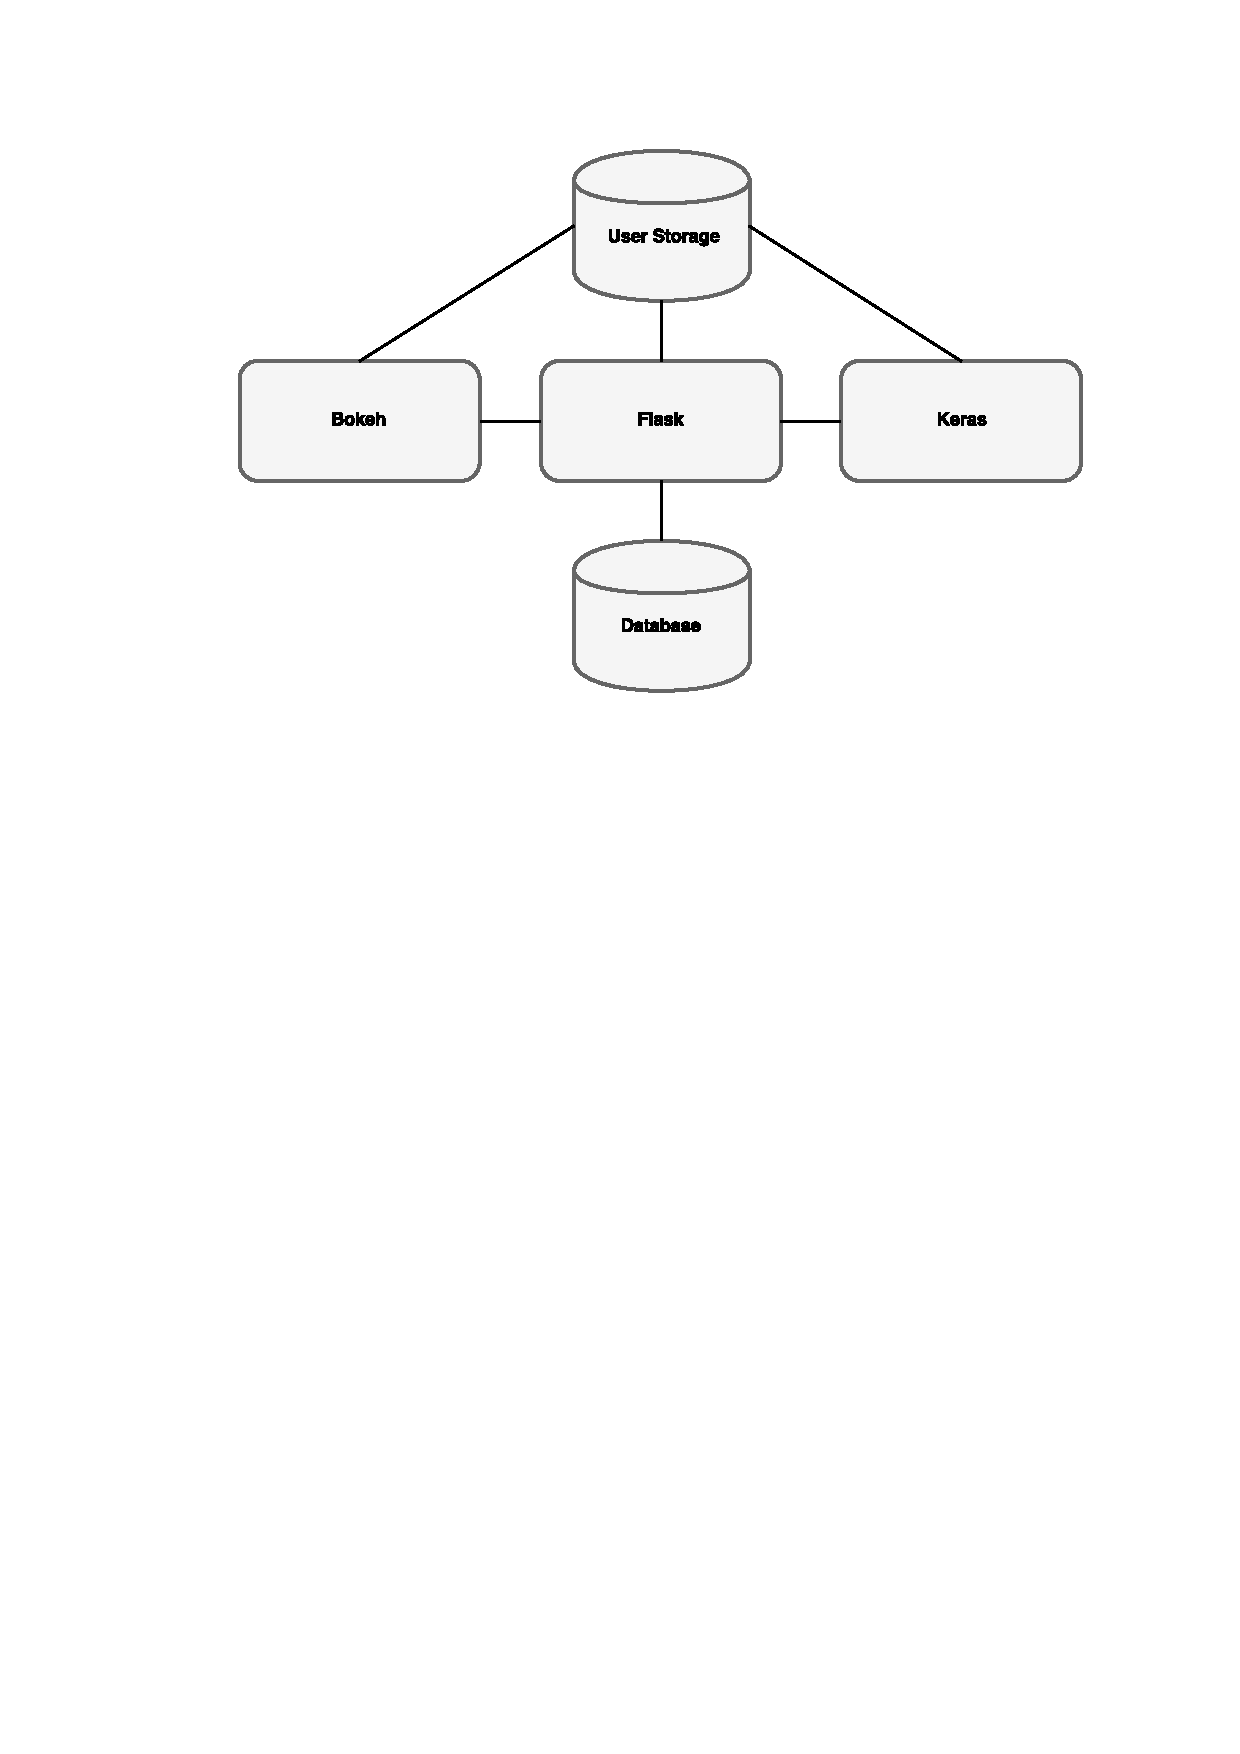
\includegraphics[width=0.8\textwidth]{fig/overall-architecture.pdf}
        \caption{Overall Architecture of the System}
        \label{architecture1}
\end{figure}

\begin{figure}[h!]
    \centering
        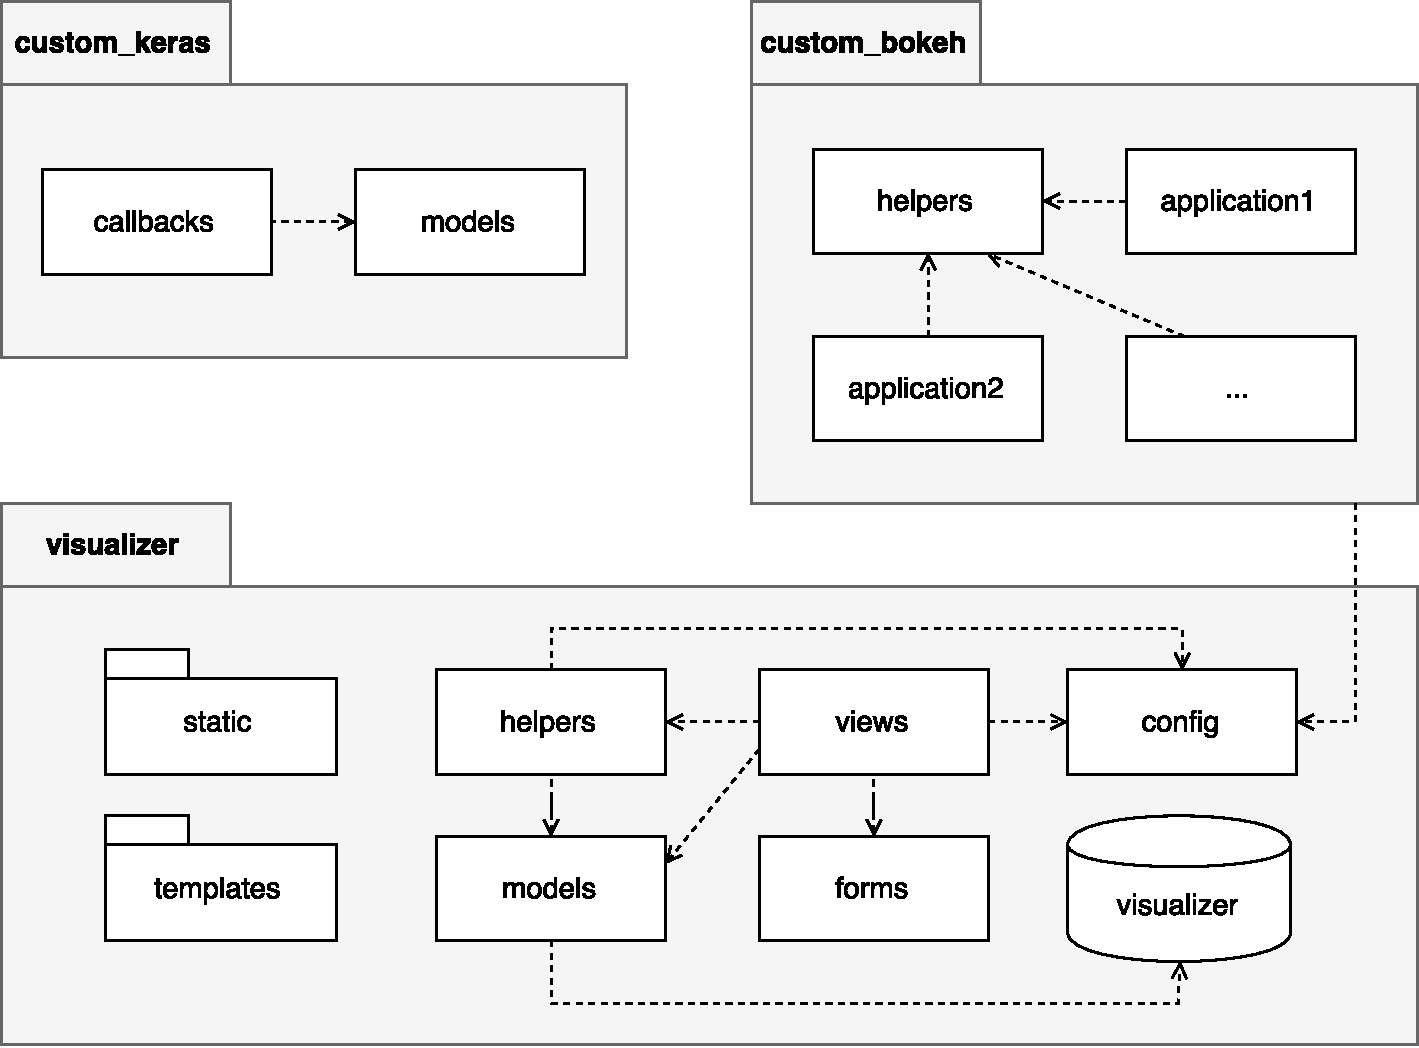
\includegraphics[width=\textwidth]{fig/package-diagram.pdf}
        \caption{Package Diagram}
        \label{architecture2}
\end{figure}

% Examples here are the relation between bokeh and flask, flask and keras, flask and the user storage. etc.

\subsection{The Flask Application}

\textbf{Fig. \ref{struct}} shows an overview of the structure of the files included in the Flask application. The static folder serves all the CSS and JavaScript files, while the templates folder contains Jinja2 templates that Flask can render to generate the HTML. The init file contains the instantiation of the Flask application as well as some setup for the database and log in system. The config file configures some parameters for the application, such as the command used to run a python script.\\

\begin{figure}[h!]
\begin{verbatim}
/visualizer
    /static
        /css
        /fonts
        /js
    /templates
        /create_user.html
        /home.html
        /layout.html
        /...
    /__init__.py
    /config.py
    /forms.py
    /helpers.py
    /models.py
    /requirements.txt
    /views.py
    /visualizer.db
\end{verbatim}
\caption{Flask project files}
\label{struct}
\end{figure}

\noindent There are three main files implementing the logic: forms.py, models.py and views.py. They define all the forms, models and views, respectively, of the web page. A form is used to collect user input, for instance while registering a new user, or uploading a script. Models are used to create database objects. Finally, a view defines a URL endpoint, or a route, as well as what HTTP requests it answers to, and determines what should happen when a user arrives at that URL. There is also a helpers file that contains various helper methods.\\

\noindent An actual example of a view from views.py is shown in \textbf{Code \ref{code:2}}. Comments and irrelevant code are removed to simplify the example. Line 1 defines the route of the view, hence the complete URL of this view will be \texttt{localhost:5000/create\_user}. It also defines the HTTP requests to answer to, which is both GET and POST. GET is for just returning the page to register a user, while POST is when a user actually presses the button to register. The code illustrates the use of a form in line 3, in this case a form for creating a new user, which contains the chosen username and password of the new user. Line 5 checks if all fields are valid when a user has submitted (the POST request), while the next line makes sure to alert the user and break the process if the username is already taken. If everything this far is fine, line 9 creates a User model consisting of the username and password (the model also takes care of hashing the password) and adds it to the database. Line 13 redirects the user to another view, namely the log in view. If the user has not submitted their form, line 15 makes sure to render the correct template for the user registration page. \\

\begin{listing}[h!]
\begin{minted}
[
frame=lines,
framesep=2mm,
baselinestretch=1.2,
fontsize=\footnotesize,
linenos
]
{python}
@app.route('/create_user', methods=['GET', 'POST'])
def create_user():
	form = CreateUserForm()
	
	if form.validate_on_submit():
		if not unique_username(form.username.data):
			flash('Username is already taken', 'danger')
		else:
			db.session.add(User(form.username.data, form.password.data))
			db.session.commit()
			
			flash('User successfully created', 'success')
			return redirect(url_for('login'))
		
	return render_template('create_user.html', form=form)
\end{minted}
\caption{View for creating a user}
\label{code:2}
\end{listing}

\subsection{Database}

As mentioned earlier, the database is very simple, and does not play a huge role in the implemented application. Its purpose is to handle the user system and store useful meta data about the uploaded scripts. It consists of three models, with attributes and connections as seen in \textbf{Fig. \ref{database}}. The \texttt{User} model contains necessary information of a user. The \texttt{FileMeta} model contains the meta data of the scripts, as well as a connection to its owner. There is also a separate \texttt{Tag} model, that can be associated to zero, one, or several scripts.

\begin{figure}[h!]
    \centering
        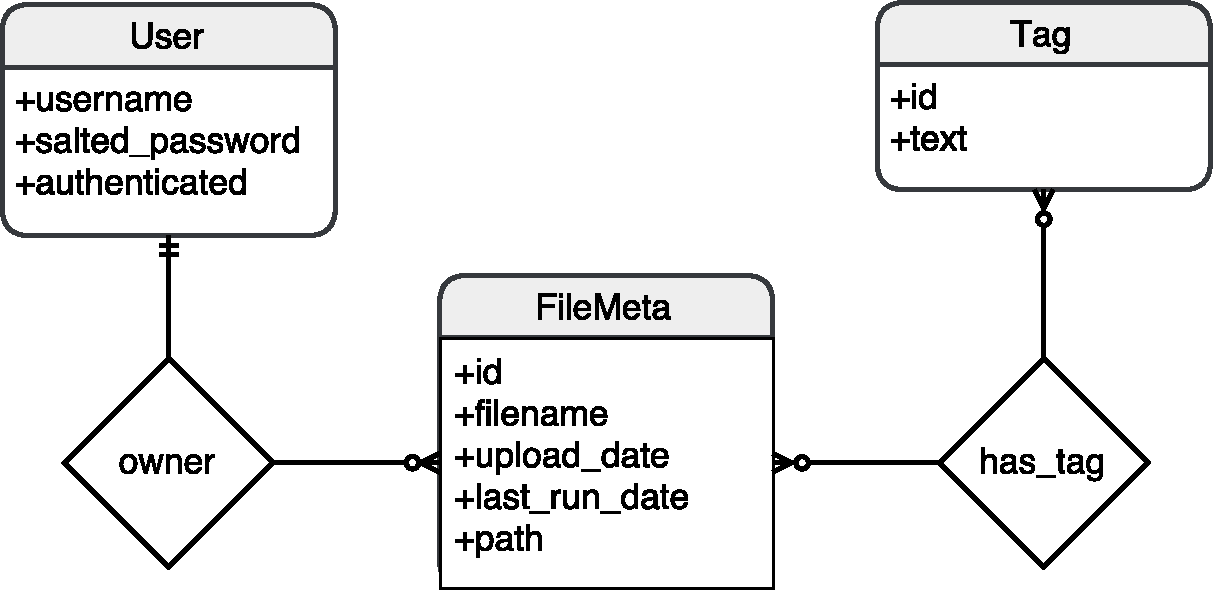
\includegraphics[width=0.7\textwidth]{fig/database-diagram.pdf}
        \caption{ER-diagram of the database}
        \label{database}
\end{figure}

\subsection{User Storage}

The user storage is where the scripts are uploaded to, and where the training data is stored. The structure of the user storage can be seen in \textbf{Fig. \ref{struct2}}. The top level holds the different users of the system. The second level contains the various scripts that a user has uploaded. At the next level, the script-file itself is stored, as well as a text file containing the output of a run of the script. There is a folder called 'images' that contains the image that the user has uploaded to be used in the visualizations. The 'networks' folder contains the most currently saved network created by the script. The folder called 'results' stores all the data produced by the various callbacks. The files are all given descriptive names so that it is self-evident which file corresponds to which visualization technique.

\begin{figure}[h!]
\begin{verbatim}
/user-storage
    /<user1>
        /<script1>
            /images
                /<image>
            /networks
                /<network>
            /results
                /deconvolution_network.pickle
                /deep_visualization.pickle
                /layer_activations.pickle
                /saliency_maps.pickle
                /training_progress.txt
                /training_progress_val.txt
            output.txt
            <script1>
        /<script2>
            /...
    /<user2>
        /...
\end{verbatim}
\caption{User storage structure}
\label{struct2}
\end{figure}

\subsection{Running a Python Script}

The visualization tool allows a user to both start and stop the uploaded python scripts. Functionality for running a script is implemented as a helper function, and is done by executing \texttt{python [file\_path]} in a new subprocess, as seen in \textbf{Code \ref{code:3}}. The actual Python command is determined by a config variable, since it depends on the user's Python installations (e.g. some systems use \texttt{python3} for Python 3.6 and simply \texttt{python} for Python 2.7). The \texttt{stdout} argument specifies the standard output file handle, which is in this case a text file that will be displayed on the web page, so that the user is given easy access to the output of the script. Note that even though \textbf{Fig. \ref{architecture1}} shows a connection between Keras and Flask, the real connection is really between Python and Flask. A user could easily upload a Python script that uses the scikit-learn library or pure TensorFlow, running such a script would not cause any problems. However, if someone wanted to adapt the visualization tool to a whole different programming language, this section of the code would need to be replaced.

\begin{listing}[h!]
\begin{minted}
[
frame=lines,
framesep=2mm,
baselinestretch=1.2,
fontsize=\footnotesize,
]
{python}
with open(get_output_file(get_current_user(), basename(file_path)), 'w') as f:
	p = subprocess.Popen([PYTHON, file_path], stdout=f)
\end{minted}
\caption{Running a Python script using subprocess}
\label{code:3}
\end{listing}

\subsection{Custom Keras Callbacks}

The custom callbacks are the only part of the visualization tool that are specific to Keras. As mentioned, a callback is a set of functions to be applied at given stages of the ANN training procedure, and Keras provides the user with many of these including the possibility of creating your own callbacks. We have taken advantage of this functionality, and created a callback for each visualization technique, as well as some other useful functionality to be utilized on the web page. An overview of all of them, and how to adapt them to your script, is thoroughly explained in the appendix. In addition, we we will also showcase some of the implementation in this section.

\subsubsection{CustomCallbacks - A Wrapper Class for the Callbacks}

All of our custom callbacks require the path to the correct folder in the user storage where all of the training data needed should be written. There are also some optional arguments that all callbacks can take, and some of the callbacks require and provide their own optional or non-optional arguments, such as a list of neurons to be visualized, or a list of layers to be excluded from the visualization. To simplify the user's process of adding callbacks to their code, we created a wrapper class that takes all the common arguments on its instantiation. The wrapper class also provides methods for registering each callback with their associated arguments, and a method for getting the list of registered callbacks. A user can apply their selected calbacks by passing this list to the \texttt{.fit()} method of a Keras model.\\

\noindent An excerpt of the implementation of the wrapper class is shown in \textbf{Code \ref{code:4}}. There you can see the initialization of an instance of the class, which instantiates the necessary and optional variables. The argument named \texttt{file\_folder} is the path to the folder of the script the callbacks are applied to, noted as \texttt{<script1>} and \texttt{<script2>} in \textbf{Fig. \ref{struct2}}. This is needed to know where the callbacks should store their produced data. The arguments \texttt{custom\_preprocess} and \texttt{custom\_postprocess} are functions that can be defined by the user to pre- and post-process images to be used in visualization. The argument named \texttt{base\_interval} is the interval that the callbacks are called at unless other is specified. The callbacks are of various computational size, and some of them take significantly longer to finish than others. These have their own interval argument that overrides the base interval.\\

\noindent The excerpt also shows two of the register methods of the class. The first one named \texttt{register\_training\_progress} simply created a new instance of the \texttt{Training\-Progress} callback with the already defined file folder as a parameter, and adds it to the callback list. The second method named \texttt{register\_saliency\_maps} does exactly the same thing, except that it also takes the mentioned interval argument which is specific for the \texttt{SaliencyMaps} callback. If the user has not specified such an interval, the interval of the callback is set to the base interval previously defined. The pre- and post-process functions are also passed on to the callback.

\begin{listing}[h!]
\begin{minted}
[
frame=lines,
framesep=2mm,
baselinestretch=1.2,
fontsize=\footnotesize,
linenos
]
{python}
class CustomCallbacks:

	def __init__(self, file_folder, custom_preprocess=None, 
	    custom_postprocess=None, base_interval=10):
		
		self.file_folder = file_folder
		self.custom_preprocess = custom_preprocess
		self.custom_postprocess = custom_postprocess
		self.base_interval = base_interval
		self.callback_list = []
		
	def get_list(self):
		return self.callback_list
		
	def register_training_progress(self):
		self.callback_list.append(TrainingProgress(self.file_folder))
		
	def register_saliency_maps(self, interval=None):
		if interval is None:
			interval = self.base_interval
		self.callback_list.append(SaliencyMaps(self.file_folder, 
		                                        self.custom_preprocess, 
		                                        self.custom_postprocess, 
		                                        interval))
\end{minted}
\caption{Wrapper class for custom callbacks}
\label{code:4}
\end{listing}

\subsubsection{Example Implementation of a Callback}

The implementation of the \texttt{LayerActivations} callback can be seen in \textbf{Code \ref{code:5}}. Specific functionality is removed, as the purpose is to showcase the general approach. The callback is an extension of the base abstract class \texttt{keras.callbacks.Callback} as you can see in line 1. The initialization takes all necessary and optional arguments, and set the attributes accordingly. The folder to save the data is obtained by taking the \texttt{file\_folder} argument and adding 'results' to it. Line 13 starts the process of getting the visualization image and converting it to the correct format. In line 18, the preprocess function is applied if the user has specified one. \\

\noindent The Keras callbacks provides various methods that are called at specified events, such as \texttt{on\_batch\_end} which is used in this example. Other methods used in the other callbacks are \texttt{on\_train\_begin} and \texttt{on\_epoch\_end}. The counter value is increased in line 25, and line 28 checks whether it is time to perform the computation of the visualization data. The specific functionality varies from the different visualization techniques, and will not be further explained. Finally, line 32 creates the correct file for storing the data, in this case in a pickle file, and the counter is reset. Note that some of the callbacks also takes use of a postprocess function, which would be applied to the result before saving it.

\begin{listing}[h!]
\begin{minted}
[
frame=lines,
framesep=2mm,
baselinestretch=1.2,
fontsize=\footnotesize,
linenos
]
{python}
class LayerActivations(Callback):

	def __init__(self, file_folder, exclude_layers=EXCLUDE_LAYERS, 
	               custom_preprocess=None, interval=10):

		super(LayerActivations, self).__init__()
		self.results_folder = join(file_folder, 'results')
		self.interval = interval
		self.counter = 0

		self.exclude_layers = exclude_layers

		images_folder = join(file_folder, 'images')
		img_name = listdir(images_folder)[-1]
		img = Image.open(join(images_folder, img_name))
		self.img_array = img_to_array(img)

		if custom_preprocess is not None:
			self.img_array = custom_preprocess(self.img_array)
		
		self.img_array = np.expand_dims(self.img_array, 0)

	def on_batch_end(self, batch, logs={}):

		self.counter += 1
		layer_tuples = []

		if self.counter == self.interval:

			# specific functionality, removed to simplify example

			with open(join(self.results_folder,
			                'layer_activations.pickle'), 'wb') as f:
				pickle.dump(layer_tuples, f)

			self.counter = 0
\end{minted}
\caption{Example implementation of a callback}
\label{code:5}
\end{listing}

% can add more specifics for the callbacks here, either in a subsubsection or in a new subsection???

\subsection{The Bokeh Server}

The visualizations are displayed in the user interface utilizing the Bokeh visualization library. The most flexible approach of embedding these in Flask is to make use of the Bokeh Server. A Bokeh application is created for each visualization technique, and these are served by the server using the \texttt{bokeh serve [applications]} command, where applications is a list of paths to the various applications, separated by spaces. The server uses the application code to create sessions and documents. A document is Bokeh's organizing data structure containing all the models and data needed to render the application in the browser.\\

\noindent The Bokeh Server is embedded into the code of the Flask application as seen in \textbf{Code \ref{code:6}}. This method is called whenever a user selects a tab that contains a visualization. \texttt{app\_path} is the corresponding relative path to the selected visualization, for instance 'training\_progress'. The full URL of the training progress Bokeh application is thus \texttt{BOKEH\_SERVER}, which is the URL of the server imported from the config file, joined together with \texttt{app\_path}. The server is loaded in line 3, returning a script tag that will replace itself with a Bokeh plot when placed in a HTML template. The Bokeh application will need to know the filename and the username in order to locate the correct visualization data file that should be visualized. Bokeh allows for passing HTTP request arguments to its applications, but has not yet implemented a way of passing these in \texttt{autoload\_server}. Therefore, we need to manually insert the filename and username into the script tag, as seen in line 5 through 11. Finally, the script can be returned and is further passed on to a HTML template. The complete process, starting from a user clicking on one of the visualization tabs, to the user actually viewing the visualization, is illustrated in a sequence diagram in \textbf{Fig. \ref{bokeh-server}}.

\begin{listing}[h!]
\begin{minted}
[
frame=lines,
framesep=2mm,
baselinestretch=1.2,
fontsize=\footnotesize,
linenos
]
{python}
def get_bokeh_plot(filename, app_path):

	script = autoload_server(model=None, url=urljoin(BOKEH_SERVER, app_path))

	params = {'user': get_current_user(), 'file': get_wo_ext(filename)}
	
	script_list = script.split('\n')
	script_list[2] = script_list[2][:-1]
	script_list[2] += '&' + urlencode(params) + '"'
	
	return '\n'.join(script_list)
\end{minted}
\caption{Embedding the Bokeh server in Flask}
\label{code:6}
\end{listing}


\begin{figure}[h!]
    \centering
        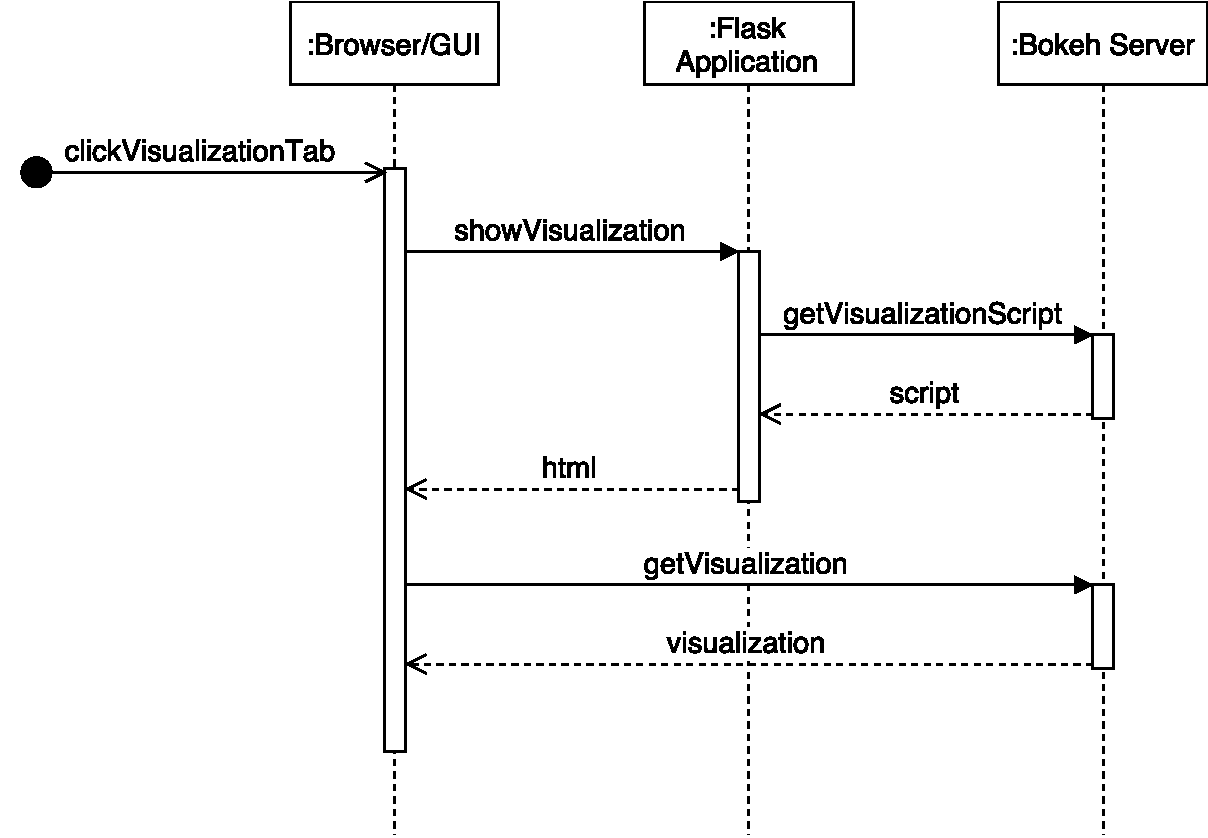
\includegraphics[width=\textwidth]{fig/sequence-bokeh.pdf}
        \caption{Sequence diagram of getting a visualization from Bokeh Server}
        \label{bokeh-server}
\end{figure}

\subsection{Bokeh Applications}

As mentioned, a Bokeh application is created for each visualization techniques, which gives the following five applications:

\begin{itemize}
    \item deconvolution\_network.py
    \item deep\_visualization.py
    \item layer\_activations.py
    \item saliency\_maps.py
    \item training\_progress.py
\end{itemize}

The implementation of the applications are quite different, and we will not describe them all in detail. Rather, we will present some of the most important concepts of the implementations. The resulting visualization can be seen in the results chapter.

\subsubsection{Handling the Visualization Data}

All of the Bokeh applications begins with the same lines of code, shown in \textbf{Code \ref{code:7}}. The document variable in line 1 holds the current Bokeh document that we are working on. In lines 2-5, we get the HTTP request arguments from the request from the Flask application. These arguments are used to find the path in the user storage corresponding to the file we are going to visualize data for, as in line 7. \texttt{UPLOAD\_FOLDER} is the path to the upload folder, imported from the config file. Some of the Bokeh applications also display the original image used in the visualization. This image is found using the same method as for the visualization files. \\

\begin{listing}[h!]
\begin{minted}
[
frame=lines,
framesep=2mm,
baselinestretch=1.2,
fontsize=\footnotesize,
linenos
]
{python}
document = curdoc()
args = document.session_context.request.arguments

file = args['file'][0].decode('ascii')
user = args['user'][0].decode('ascii')

results_path = join(UPLOAD_FOLDER, user, file, 'results')
\end{minted}
\caption{Getting the data from the visualization files}
\label{code:7}
\end{listing}

\noindent The data loaded from the visualization file is processed to a format that it can be displayed in. The processing depends on the specific visualization technique. For instance, data for the training progress is transformed into separate sequences of x- and y-values. The other techniques mostly output images, and the image data needs to be converted into 2D arrays, since Bokeh does not handle 3D arrays for images. For layer activations, the results include several smaller images. These are stitched together into a grid of images for each layer. When the data is properly processed, it is stored in a ColumnDataSource, an object that stores data to be used in a Bokeh figure. In our case, its main purpose is to allow for simple streaming of data. When associating a ColumnDataSource with a figure, updating the data of the ColumnDataSource automatically triggers an update of the figure. This is much more effective than creating a new figure every time the data is updated.


\subsubsection{Callbacks}

% first couple of lines of the code
% column data sources
% callbacks


\section{Case Study in Face Recognition}

\textit{Describe the case study (facial recognition with expression).
Should already be presented, but here we can add specifics, and also possibly describe the structure of the network we have created, the dataset used, etc.}

\subsection{Method}

% probably should write something about how we have been working? corresponding to the system development method in the visualization tool section.


\subsection{Pretrained Model}

As described in section X.X, transfer learning is a convenient method for training an ANN without requiring long training periods or large amounts of training data. This can be done by using a pretrained model. Since our case study deals with face recognition, it is beneficial to use a CNN trained on images of faces. Such a network would already be able to detect specific features like eyes and mouths. A suitable model is the VGG-Face CNN described in section X.X. The original implementation is using Caffe, but luckily a Keras implementation converted from the original Caffe network can be found available for download. We plan to employ transfer learning using this network as the pretrained model.

% CNN trained on faces
% something that is available for Keras
% https://github.com/rcmalli/keras-vggface

\subsection{Dataset}

Based on the restrictions regarding the dataset described in section X.X, as well as the exploration of potential datasets conducted in the Specialization Project, the Indian Movie Face database (IMFDB) was selected. This database consists of 34,512 images of 100 actors collected from Indian movies, captured in an unconstrained setting. All images are selected and labeled manually, including both of our required labels, namely identification and expression. The available expressions are the six basic expressions described in section X.X, in addition to a neutral expression, giving a total of seven possible values for the expression label. The dataset is structured so that it contains a folder for each of the actors. These folders again contain a folder for each movie the images of the actor is taken from. A movie folder contain and image folder, and a text file with all image names and their corresponding labels. \\

\noindent After downloading the dataset, we received some errors while trying to process the text files. Thus, we created a script that traversed the text files of the dataset and alerted us of any peculiarities. Some of the entries were missing their expression labeling and these were removed entirely. Others were just improperly formatted, so that they were easily fixed. This process slightly reduced the size of the training set, resulting in a dataset with XX,XXX images of XX actors.

% suitable in terms of size
% similar to images vgg16-face is trained on?
% available for download and free of charge
% skrive at det ikke har dukket opp noen nye

\subsection{Preprocessing of Data}

% images were already cropped
% padded and resized.

\subsection{Architecture}

% network architecture (for alle 2-3)
% skrive om hvordan vi har brukt transfer learning



\cleardoublepage